



\chapter{Einleitung}

\begin{center}
    \begin{figure}[h]
        
\includegraphics[width=\textwidth]{img/PIA23645_PaleBlueDotRevisited_1600.jpg}
        \caption{``The Pale Blue Dot'' Feb. 14, 1990, by NASA\footnotemark.}
        \label{fig:my_label}
    \end{figure}
    \footnotetext{\fullcite{nasa.bluedot}}
\end{center}

''Ein Bild sagt mehr aus als tausend Worte.`` Dieses bekannte Sprichwort drückt aus, wie mächtig Bilder als Kommunikationsmittel sind.
Bilder beinhalten Informationen, vermitteln Emotionen, erzählen Geschichten und sind ein Fenster in die Vergangenheit.
Bilder sind in der modernen Gesellschaft omnipräsent und im Alltag digital als auch analog unentbehrlich.

Bilder unterscheiden sich je nach Aufnahme in den verschiedenen Eigenschaften ihrer Speicherung und Darstellung.
Zwei dieser Eigenschaften sind die Größe und die Auflösung eines Bildes.
Die Größe eines digitalen Bildes gibt an, wie viele Pixel es enthält, während die Auflösung eines Bildes angibt, wie viele Pixel pro Flächeneinheit vorhanden sind (PPI). %TODO Wollen wir ein Abkürzungsverzeichnis? 
Die Größe und die Auflösung eines Bildes haben Einfluss auf seine Qualität und seinen Speicherplatzbedarf.
Um ein Bild für einen bestimmten Zweck zu nutzen, muss es häufig in seiner Größe und oder Auflösung verändert werden.
Der Vorgang zur Veränderung der Größe und Auflösung wird als Bildskalierung bezeichnet\footfullcite{techlib.scaling}\footfullcite{abcdef.scaling} und ist eine grundlegende Operation in der digitalen Bildverarbeitung.

Bildskalierung ist eine grundlegende Methode der Bildverarbeitung. Bildskalierung erlaubt die Änderung der Größe eines digitalen Bildes.
Eine Gute Bildskalierung misst sich an ihren Eigenschaften in den Bereichen Rechenaufwand und Qualitätsverlust.
Besonders wichtig ist der Qualitätsverlust, wenn man Bilder größer skaliert.
Ein geeignetes Modell um diesen Prozess zu erklären ist das übertragen einer Zeichnung von einem kleinen Papier auf eine große Leinwand.
Wird die Zeichnung lediglich unbedacht vergrößert, wird diese unscharf und verliert an Details.
Das Ziel einer guten Bildskalierung ist es, diesen Effekt zu verhindenr und die Zeichnung größenunabhängig scharf und detailreich darzustellen.

Es gibt viele verschiedene Methoden, um die Größe eines Bildes zu ändern.
Klassische Methoden verwenden Interpolationstechniken, die neue Pixel aus den vorhandenen Pixeln berechnen.
Diese Methoden sind schnell und stellen einen geringen Rechenaufwand in Kombination mit geringer Komplexität dar.
Jedoch kommt es mit diesen Algorithmen oft zu Qualitätsverlusten oder der Erzeugung von Artefakten.
Moderne Anwendungen zur Skalierung von Bildern verwenden Deep-Learning-Techniken wie Convolutional Neural Networks (CNNs) oder Generative Adversarial Networks (GANs), die neue Pixel aus einem trainierten Modell erzeugen.
Diese neuen Methoden sind komplex und benötigen mehr Rechenaufwand, können allerdings die Qualität des Bildes verbessern oder kreative Effekte erstellen.

\begin{figure}[h!]
    \vspace{8mm}
    \centering
    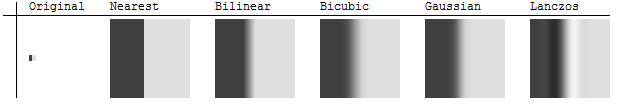
\includegraphics{img/xaR8r.png}
    \caption{Verschiedene Beispiele von upscaling Algorithmen\cite{whuber.lanczos}.}
    \label{fig:my_label}
    \vspace{4mm}
\end{figure}

Die Bildskalierung hat heute viele Anwendungen in verschiedenen Bereichen wie beispielweise Webdesign, Fotografie, Druck oder Videotechnik.
Es gibt auch in modernen Anwendungen verschiedene Arten von Skalierungsverfahren, die sich in ihrer Funktionsweise und ihrem Ergebnis unterscheiden.
Diese Arbeit schafft einen Überblick über klassische und moderne Skalierungsverfahren sowie deren ihre Vor- und Nachteile.
Diese werden anhand von Beispielen inszeniert.
Zuletzt wird basierend auf der Evaluierung der verschiedenen Verfahren eine Empfehlung für die beste Skalierungsmethode für verschiedene Bildtypen geben.

In dieser Arbeit geht es darum herauszufinden, welche Methode zum Vergrößern oder Verkleinern von Bildern das beste Gleichgewicht aus Komplexität, Rechenaufwand und Ergebnissen liefert.
Des weiteren werden die Kriterien zur Bewertung von solchen Methoden umschrieben.
%TODO mit dem Abschnitt bin ich noch nicht happy
Dazu erklären wir zuerst die wichtigsten Konzepte der digitalen Bildverarbeitung und der Skalierung von Bildern und zeigen einige Beispiele für ihre Anwendung. Danach stellen wir die traditionellen Skalierungsmethoden vor und vergleichen ihre Stärken und Schwächen. Dann zeigen wir die neueren Skalierungsmethoden und vergleichen ihre Stärken und Schwächen. Zum Schluss bewerten wir die verschiedenen Methoden mit verschiedenen Maßstäben für die Bildqualität und geben eine Empfehlung für die beste Methode. Wir fassen unsere Ergebnisse zusammen und besprechen ihre Bedeutung und Einschränkungen.
%----------------------
